\subsection{Architecture}
% 

The issue with this approach is that Alice needs to fully trust the exchange she chose. The exchange has full control over Alice's funds since she deposited the Bitcoins until she withdraws the Ether. In the case that the exchange is attacked by hackers or is not protecting users' funds properly, Alice may never get her money back. The reputation of an exchange may provide little guidance on what exchange is trustworthy, but it is not a definite measure. In the aforementioned case of Mt. Gox, this was the most prominent exchange just weeks before its crash~\cite{Popper2014ApparentTimes}.

An alternative approach for Alice could be, that she finds a person who wants to make an opposite trade to hers. Let's further assume, that Bob wants to exchange the same amount of currency from Ether to Bitcoin and that Alice can communicate with Bob by means other than the blockchains or cryptocurrency exchanges (e.g. a cryptocurrency forum). Alice and Bob need to agree on the amounts each of them is going to transfer and they need to exchange their public addresses - namely Alice needs to give Bob her Ethereum public address and Bob needs to give Alice his public Bitcoin address. Alice then sends her Bitcoins to Bob and Bob sends her Ether to Alice. This simple transaction is illustrated in figure~\ref{fig:arch-ver0}.

\begin{figure}[ht]
    \centering
    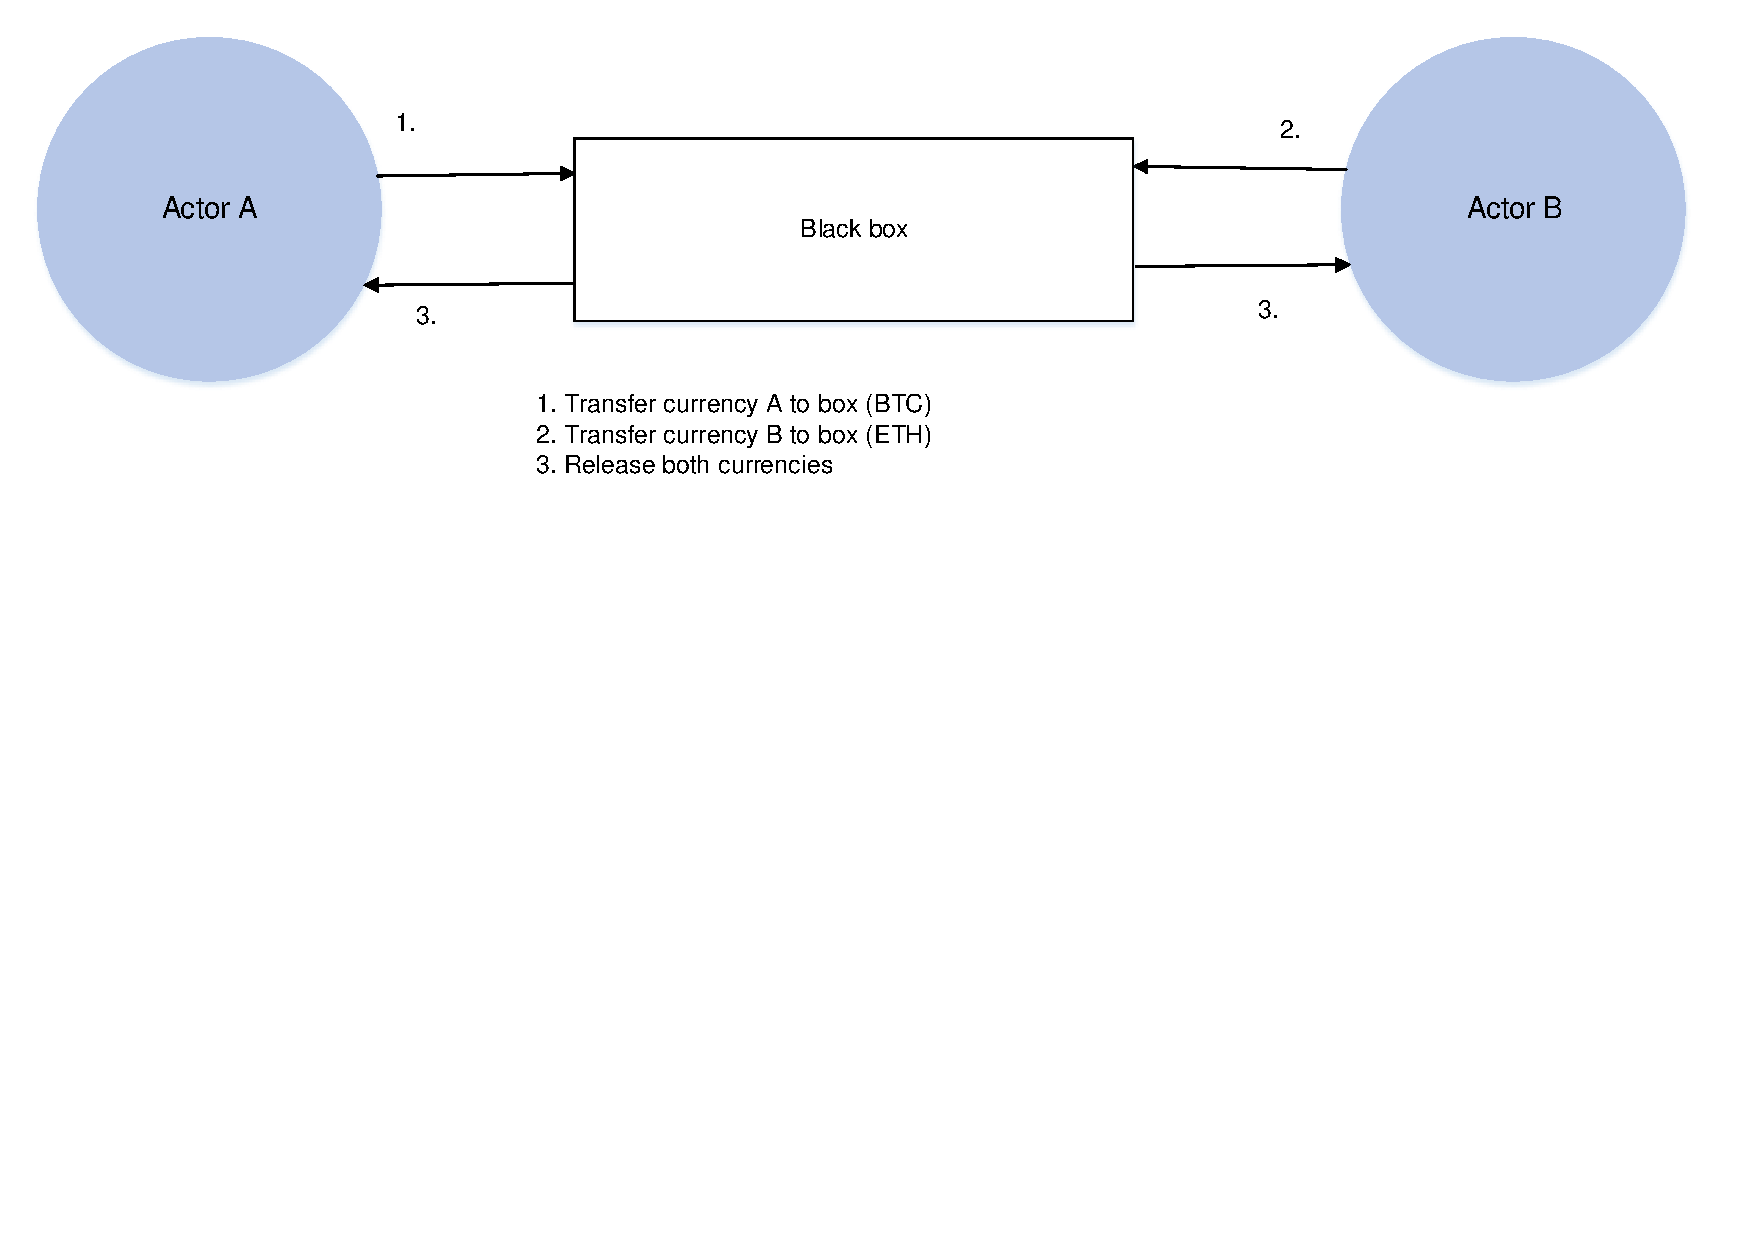
\includegraphics[width=.80\textwidth]{arch-ver0}
    \caption{The naive approach to cryptocurrency exchange. Actor A (Alice) wants to buy Bitcoin (BTC) and Actor B (Bob) wants to buy Ether. }
    \label{fig:arch-ver0}
\end{figure}

This removes the need to involve a third party in the transaction, but it does not completely solve the problem of trust. Since Alice and Bob might be located in different locations, it may be very difficult if not impossible, to ensure that the other party carries out the transaction as agreed. If Alice sends the funds to Bob, but Bob does not keep his side of the agreement and does not send his funds to Alice, it would be impossible for her to reverse the transaction. 

In an attempt to ensure that both keep their agreement, Alice and Bob could synchronise the moment when they send their transactions to the network. However, this does also not provide a fail-proof solution. For instance, Bob could subsequently send another transaction (transferring his funds to himself) from the same address, which could be processed by the network first, thus rendering the original transaction invalid.

\paragraph{Identification} 
If Alice did not receive the funds as agreed, she might want to involve traditional law-enforcement methods. But since the agreement happened over the internet, it may not be possible to successfully identify Bob.

When a reliable identification of an institution (such as an e-shop) is needed, the concept of public-key certificates has proven useful. The institution engages with a trusted third party, which then verifies the identity of this institution. Afterwards, the third party issues a certificate, that proves the identity of the institution to the visitors from the web, usually for a limited period of time~\cite{Lee2013SecurityArchitects}. 

However, for a peer-to-peer relationship, digital certificates do not seem feasible, because the process of verification of someone's identity in real world is a lengthy process. We can now see the emerging need for a system, which does not require trusting a third party, nor trusting the trading partner. In this project, we propose and implement a decentralised system running on a blockchain might be the solution to this problem. Before we present the final architecture, we will first describe on a higher-level, how such system could operate.

\paragraph{Black box architecture}
Let us introduce a `black box' between Alice and Bob. This box could hold funds from both parties and only release them under condition, that both Alice and Bob sent their respective amount. If one of them tried to cheat, the box would not release the funds further. The black box architecture is illustrated in figure~\ref{fig:arch-ver1}.
% 
\begin{figure}[ht]
    \centering
    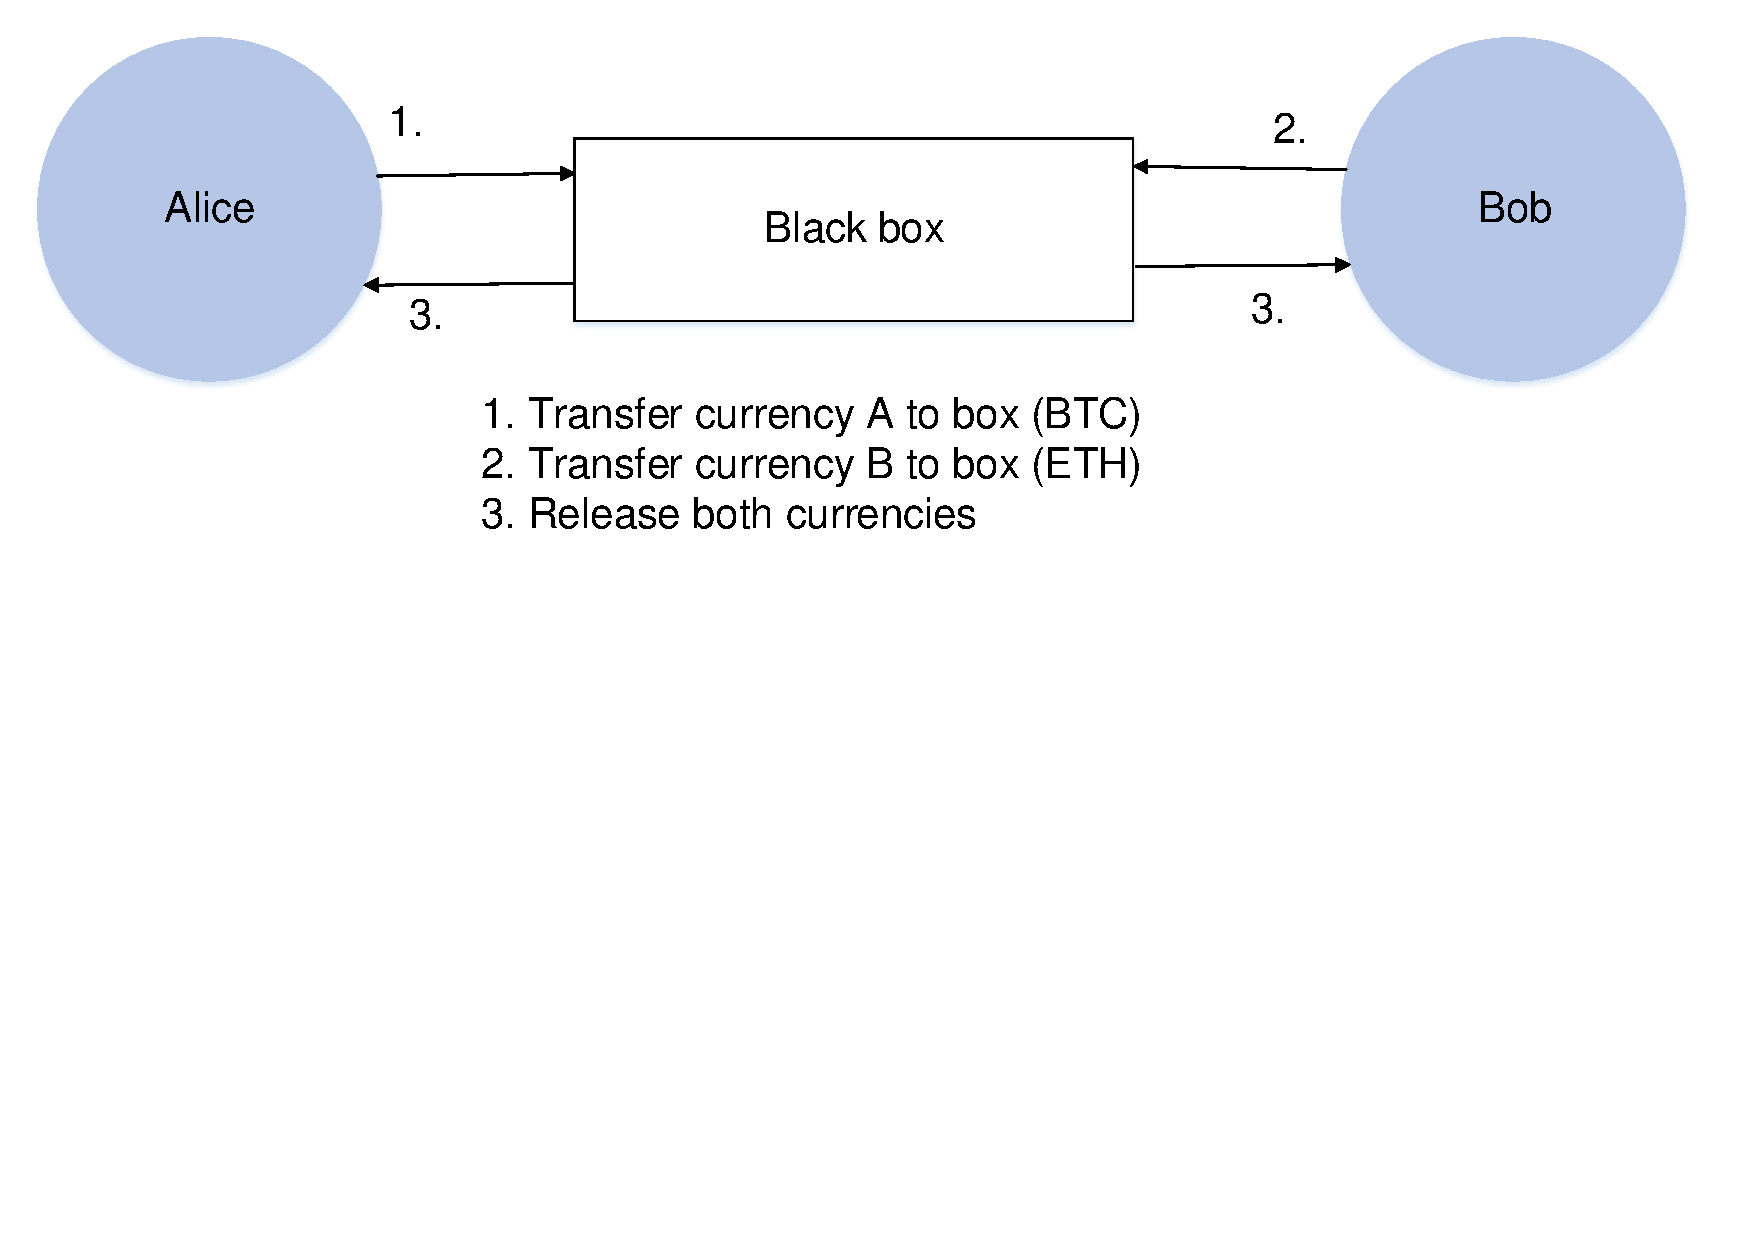
\includegraphics[width=.80\textwidth]{arch-ver1}
    \caption{Black box architecture. The black box spans both blockchains and only releases the funds, if it received the full amount from both parties.}
    \label{fig:arch-ver1}
\end{figure}

In our envisioned architecture, the black box is not a third party, rather an automated system that only operates with simple internal logic. This logic should be verifiable by anyone, however, it should not be possible to manipulate this logic by any of the parties. The black box would operate on top of both blockchains and would be decentralised. It would therefore fulfil our requirement for operation without a third party and without requiring the trading parties to trust each other.

This is a plausible architecture for a proposed system. It may be implemented on networks, that enable this kind of transaction control, either via multi-signature wallets (for example Bitcoin) or smart contracts (for example Ethereum). Another advantage is, that the parties now do not need to trust one another. In case of one party tries to cheat, the black box would not release the funds further.

The drawback of this architecture lies in technical complexity. The black box would need to operate on top of \textit{both} blockchains and would require coordination between two networks. The architecture could be simplified in order to remove the need to operate on two blockchains.

\paragraph{Half black-box architecture}
We can achieve similar functionality by only limiting the transaction control to one blockchain. This architecture could be referred to as `half black-box' and is illustrated in figure~\ref{fig:arch-ver2}. In this scenario, after initial agreement has been made, Alice proceeds to send funds to the half black-box. This transaction is public and can be verified by Bob. When Bob sees, that the funds are deposited in the box, he can now transfer his funds to Alice. The half black-box queries the blockchain for Bob's transaction in regular intervals. Once the transaction has been successfully included in the blockchain, the half black-box recognises this and can now release Alice's funds to Bob.
% 
\begin{figure}[ht]
    \centering
    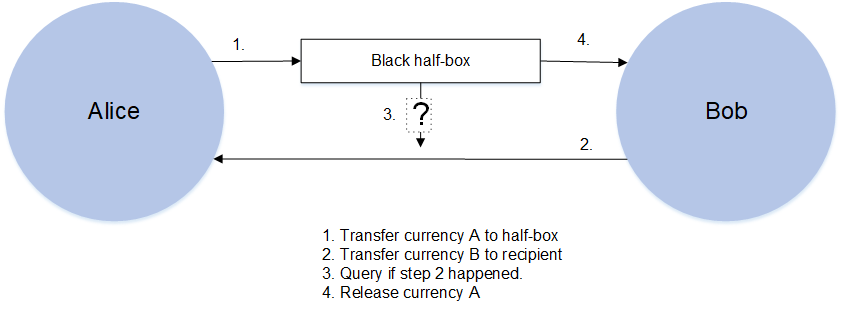
\includegraphics[width=.80\textwidth]{arch-ver2}
    \caption{Half black-box architecture. The box only controls funds on one of the blockchains. The transaction on the other blockchain happens normally. The box queries the blockchain for this transaction, and only releases the funds once it has been processed.}
    \label{fig:arch-ver2}
\end{figure}

This architecture solves the technical drawbacks of the regular black box. However, it can only work safely, if the sequence of steps is followed. In case the funds from Bob to Alice were sent \textit{before} Alice deposited her part in the half black-box, Alice is not bound to keep her part of the agreement.

The complexity of this problem lies in the design of the black half-box -- its logic needs to be verifiable by both Alice and Bob, so that both parties can engage in the transaction. As discussed earlier, the box should operate in a decentralised manner, so that there is no third party that would have control over the user's funds at any time. The logic of the half black-box would be as described in figure~\ref{fig:simple-logic}.

\begin{figure}[ht]
    \begin{framed}
    \begin{lstlisting}
class half-black-box {
	receive funds;
	check if transaction happened;
	if (transaction happened):
		forward funds to destination;
	else
		return funds to sender;
	}
    \end{lstlisting}
    \end{framed}}
    \caption{High-level notation of the logic inside a half black-box.}
    \label{fig:simple-logic}
\end{figure}


Research indicates that currently there are multiple systems that would be capable of running the logic of a black box in a decentralised manner. In our implementation we demonstrate the black box operating on the Ethereum blockchain, as the smart contracts in are capable of running such logic. This means, that Ethereum needs to be one of the two networks involved in the transaction. In this implementation, we chose Bitcoin to be the second network. We will consider other networks/currencies later. A trading scenario between Alice and Bob is illustrated in figure~\ref{fig:ethereum-case}. Figure~\ref{fig:arch-ver2-tech} provides overview of the system architecture during this scenario.

\begin{figure}[ht]
    \begin{framed}
    \textbf{Pre-conditions} Alice wants to sell Ether and buy Bitcoins. Bob wants to buy Ether and sell Bitcoins. They agree on the details of the transaction via a side channel.
 
    \begin{enumerate}[noitemsep]
        \item Alice sends Ether to the smart contract.
        \item Bob verifies this transaction.
        \item Bob sends Bitcoins to Alice.
        \item Smart contract verifies Bob’s transaction.
        \item Smart contract releases Ether to Bob.
    \end{enumerate}
      
    \textbf{Post-conditions}: Alice has Bob’s Bitcoin, Bob has Alice’s Ether.

    \end{framed}
    \caption{Trading scenario, where half black-box is implemented as a smart contract on the Ethereum network and the traded currencies are Ether and Bitcoin. Half black-box/smart contract operates the logic described in figure~\ref{fig:simple-logic}.}
    \label{fig:ethereum-case}
\end{figure}

\begin{figure}[ht]
    \centering
    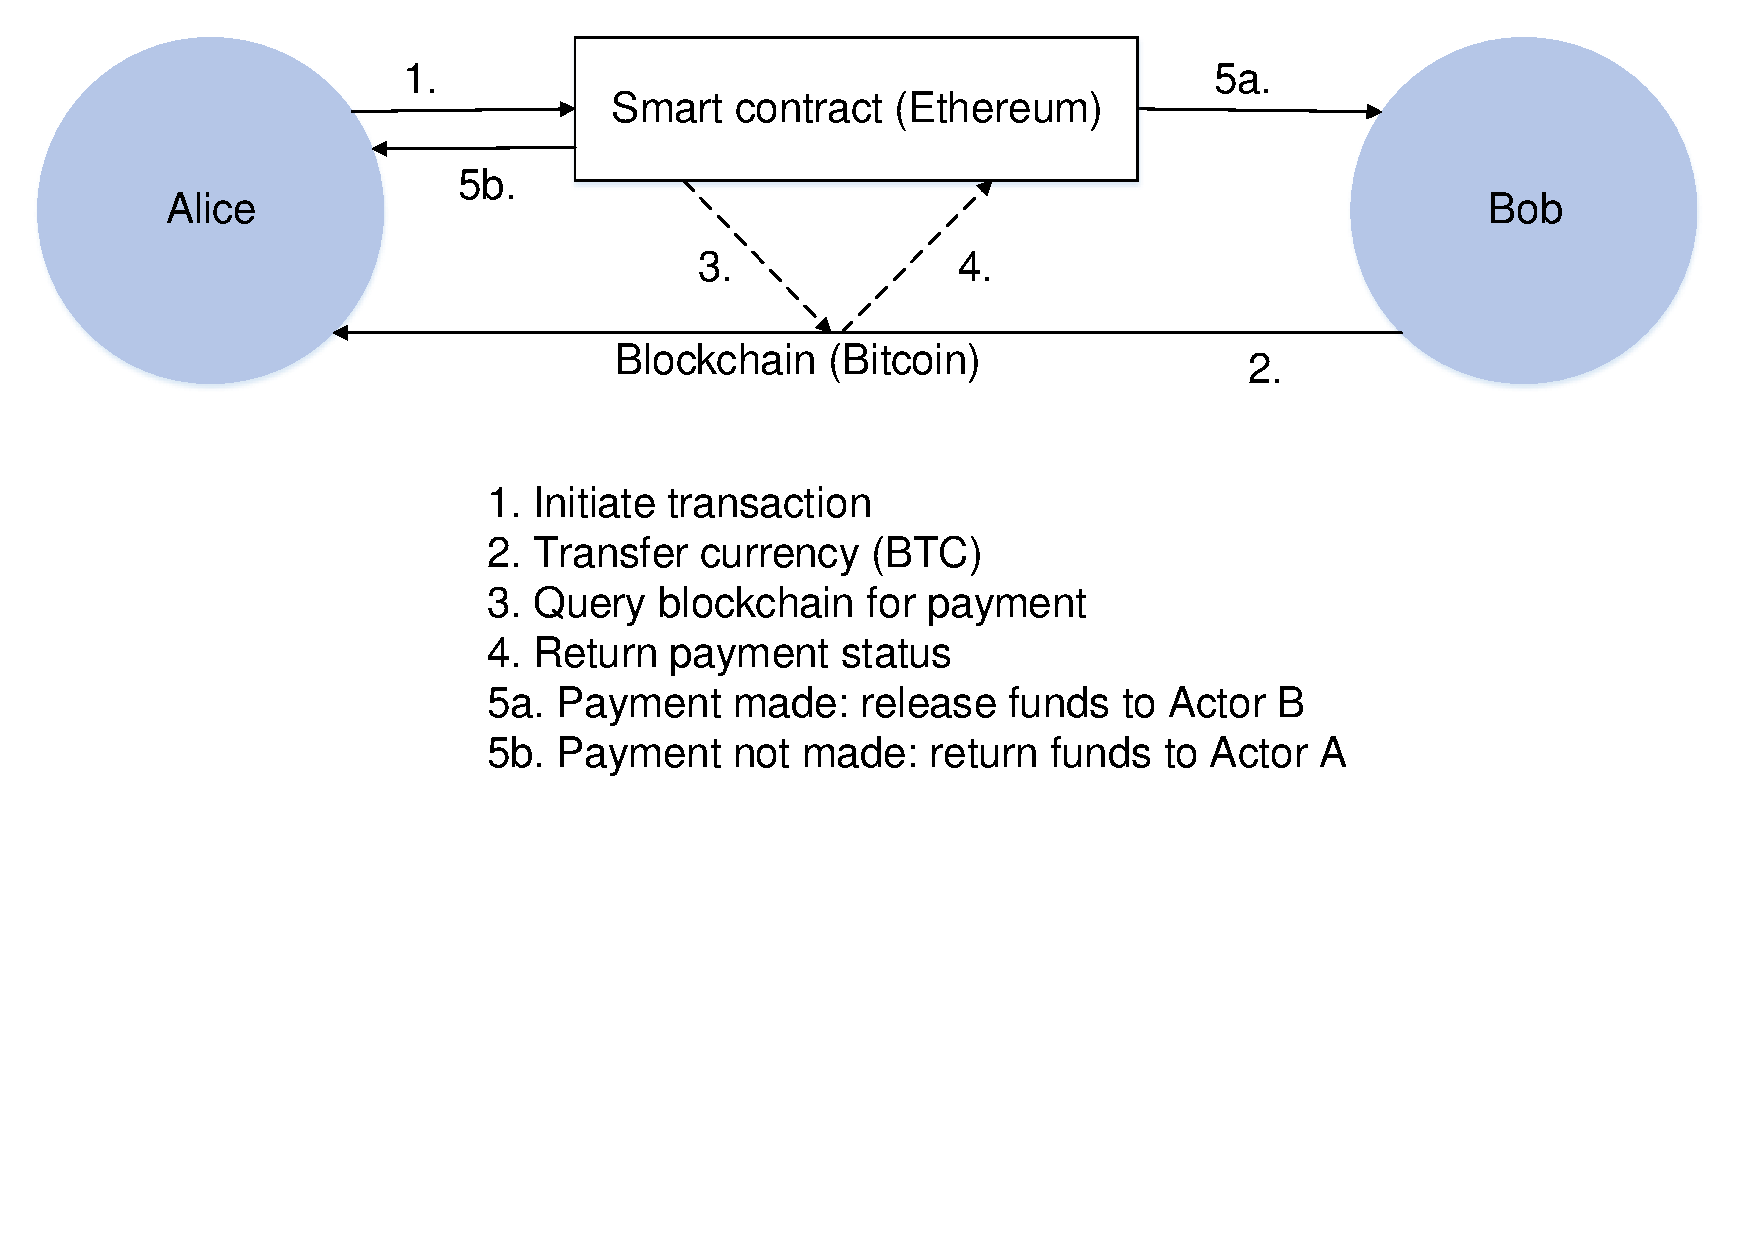
\includegraphics[width=.90\textwidth]{arch-ver2-tech}
    \caption{System architecture, reflecting the scenario in figure~\ref{fig:ethereum-case}}
    \label{fig:arch-ver2-tech}
\end{figure}

This is a high-level overview of our proposed system, but the implementation of such a system needs to resolve several fundamental issues. The first problem lies in the step number 4 of the previous scenario. Both Ethereum and Bitcoin blockchains are two separate entities, that operate on different networks and with different protocols and do not share a common communication interface. Both systems are isolated in their respective realms and do not interact during normal operation. The half black-box would reside on the Ethereum blockchain, but to verify Bob’s transaction, would need to get data from Bitcoin blockchain. Since currently there is no client that supports both blockchains and could operate on the two networks simultaneously, the half black-box needs to learn about the transaction via a shared channel.

\paragraph{Learning the state of the transaction}
Both networks operate on a peer-to-peer basis, and peers use the public internet to communicate with each other. Internet is therefore a plausible shared channel, that could be used by the half black-box to learn about the state of the transaction. There are services that allow the user to query the status of the Bitcoin blockchain by querying an own node, that is part of the network and presenting the result in a web interface or \acrshort{api}. \textit{Blockchain.info}, \textit{blockexplorer.com} or \textit{live.blockcypher.com} are examples of such services on the Bitcoin network, \textit{Etherscan.com} is an example on the Ethereum network. The half black-box could use such service to learn the status of the Bitcoin blockchain and decide to release or return the funds.

Using a particular service to fetch the data from the blockchain introduces a major drawback to our solution -- centralisation. If we rely on one particular provider to learn about a status of a Bitcoin transaction, we are exposing the system to a risk, that this provider will not provide accurate and up-to-date data, either knowingly (trying to sabotage the process) or unknowingly (by mistake). Considering scenario in figure~\ref{fig:ethereum-case}, such provider could easily halt the transaction, by providing negative answer to the query of the smart contract in step 4. This goes against the idea of a decentralised money exchange platform. A plausible solution to this problem would be to query several providers and accept the answer of the majority, to lower the possibility of an individual faulty result.

\paragraph{Inputting data to Ethereum network}
The second major problem that the system implementation needs to tackle, is the deterministic nature of the blockchain. The blockchain is built in such way, that all of the transactions need to produce the same outcome at any time. In other words, a node that joins the Ethereum network serveral years later, still needs to be able to recalculate all the transactions and reach the same outcome as the nodes do today. Consider the scenario in figure~\ref{fig:ethereum-case}, where a Node~A, executing the smart contract successfully queried the Bitcoin blockchain, learned that Bob made the Bitcoin transfer, and therefore released Ether to Alice. If a Node~B joins the Ethereum network at other time, it cannot be guaranteed that it will reach the Bitcoin blockchain and obtain the same result as Node~A. Hence, it cannot verify, whether if the release of Ether to Alice was legitimate.

The solution to this problem is provided by \textit{oracles}, which are specialised data sources that translate real-world, off-chain information into data that can be processed by the smart contract. Oracles watch the blockchain for events and respond to them by publishing the results of a query back to the smart contract~\cite{JohnWeldon2016BuildingContract}. \textit{Event} is a special type of log message, that is emitted from a contract when its state changes. Programmers can choose if and when they want to emit an event, while they write the code of the smart contract. Events can be listened for by any of the nodes, using the \code{eth\_newFilter} and \code{eth\_getFilterChanges} methods defined in the JSON-RPC specification\footnotemark, which is a standard part of commonly used nodes (such as Parity or GEth). A simple oracle could be a server that listens for these events on the Ethereum network, fetches the real-world data and then delivers them back to the contract, sending them as a part of a transaction~\cite{JulesDourlens2017Oracles:Blockchain, 2018OraclizeDocumentation}. 
% 
\footnotetext{\url{https://github.com/ethereum/wiki/wiki/JSON-RPC##eth_newfilter}, accessed 02-05-2018}
% 
\begin{figure}[ht]
    \centering
    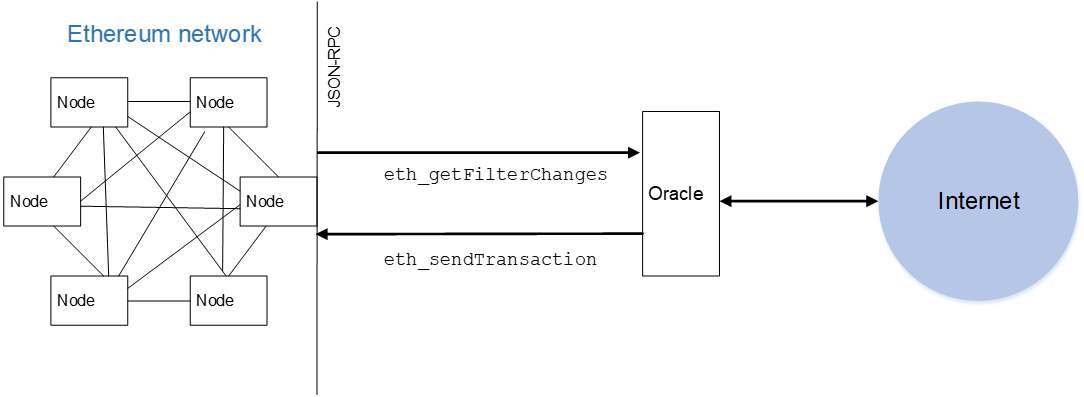
\includegraphics[width=\textwidth]{oracle-principle}
    \caption{Basic working principle of oracles. Smart contract on Ethereum network is watched for emitting an event, oracle then fetches the off-chain data from the internet and returns the result to the smart contract via a new transaction.}
    \label{fig:oracles-principle}
\end{figure}


% Regular transactions made in the Bitcoin, Ethereum, Litecoin or other coins are irreversible and once they are processed by the network, they cannot be changed. But what if a condition could be included in the transaction? A `black box' that collects funds 


% that only Some systems (Bitcoin, Ethereum) provide a functionality known as multi-signature wallets



% \begin{figure}[ht]
%     \centering
%     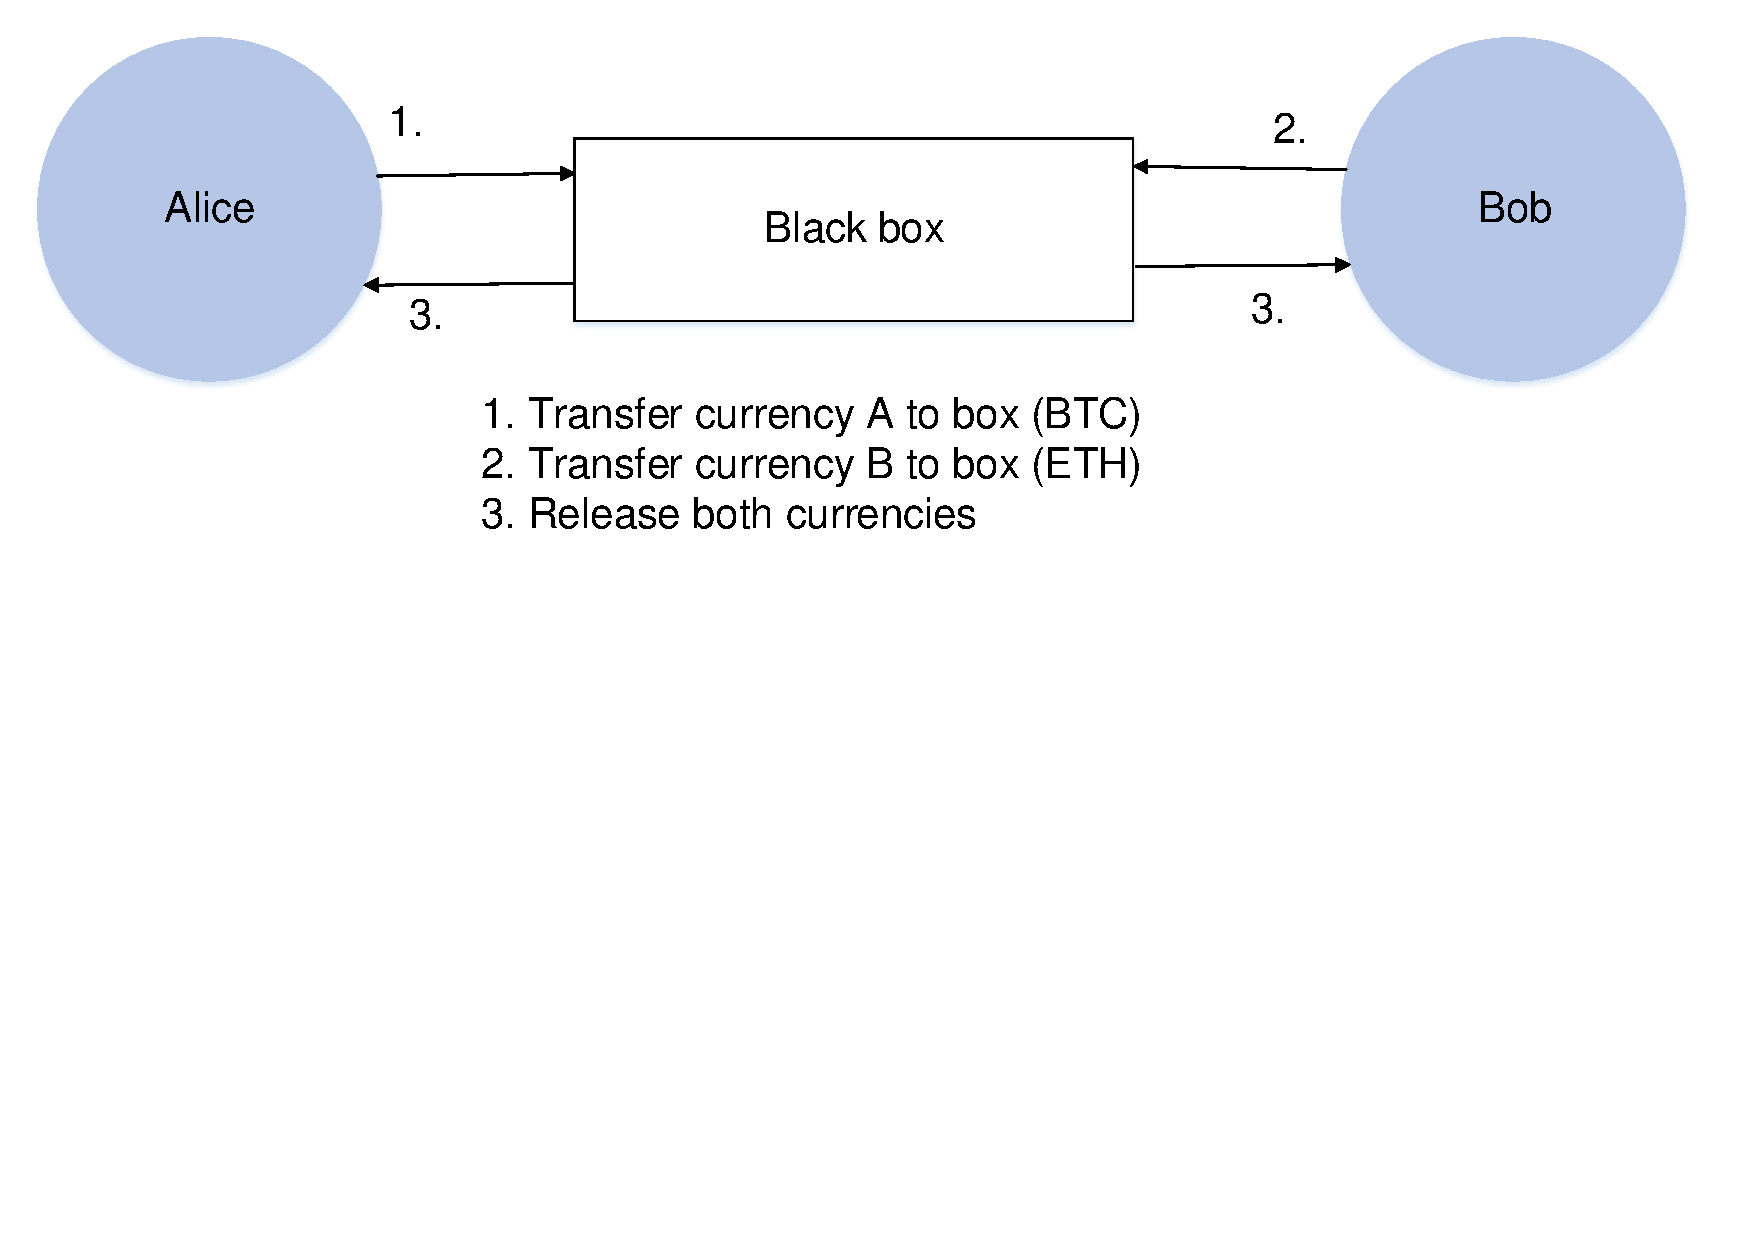
\includegraphics[width=.80\textwidth]{arch-ver1}
%     \caption{}
%     \label{fig:arch-verx}
% \end{figure}